\subsection*{Question 3.1}
In this exercise we are working on data from 40 hands, represented by 56
points on a 2D plane. One of the hands are shown in figure
\ref{fig:q31hand}, and you can se that the figure looks like are regular
hand.

With the first 40 $x$'s and $y$'s, we calculate the mean to $[1.0725, 0.4434]$ and the covariance to $[0.0039, -0.0011;
-0.0011, 0.0005]$. A visualization of the mean and covariance can be
seen in figure \ref{fig:q31onepoint}, and it can be seen that the gauss
is slightly tilted and stretched.

If we calculate the mean and covariance of all the points in the hands and
plot them together, we get a plot that represents the chance that a given
point of a hand lies in in the given area in the plot. This can be seen in
figure \ref{fig:q31allpoints}, where the plot looks like the hand itself.

\begin{figure}[!htbp]
  \centering
  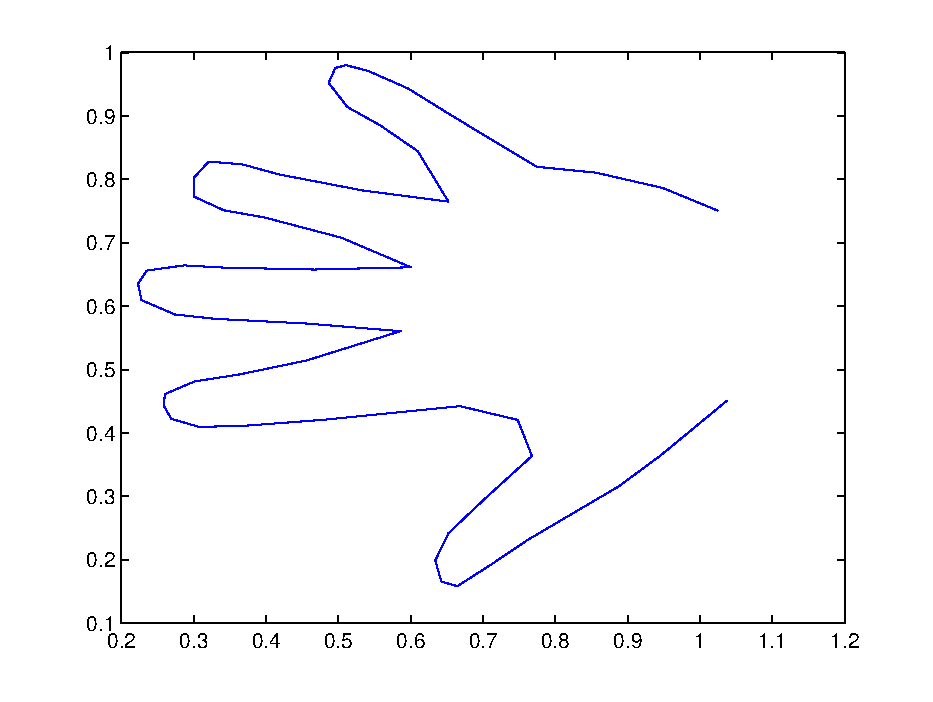
\includegraphics[width=0.85\textwidth]{./images/q31_hand}
  \caption{Shows are plot over the first hand in the data set.}
  \label{fig:q31hand}
\end{figure}

\begin{figure}[!htbp]
  \centering
  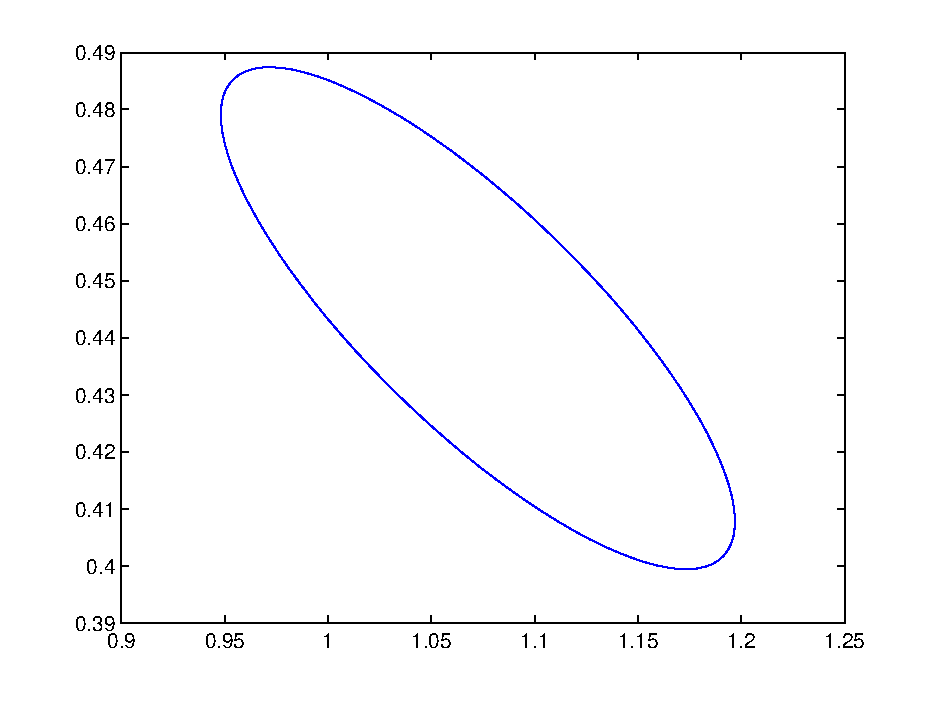
\includegraphics[width=0.85\textwidth]{./images/q31_2}
  \caption{Shows the variation of the first point of all the hands.}
  \label{fig:q31onepoint}
\end{figure}

\begin{figure}[!htbp]
  \centering
  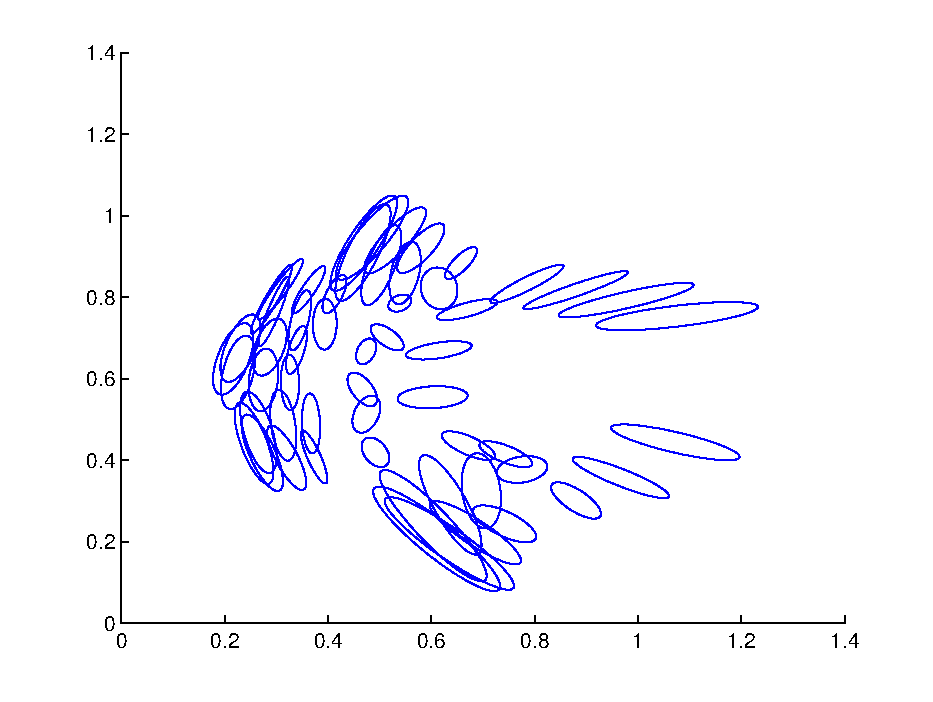
\includegraphics[width=0.85\textwidth]{./images/q31_3}
  \caption{Shows the variation of all the point of all the hands.}
  \label{fig:q31allpoints}
\end{figure}

